\section{Rappels sur les vecturs}

\begin{tikzpicture}

\draw[dashed] (-1, -1) -- (2, 2);
\draw[->, red, thick] (0, 0) -- (1, 1);
\node at (0, 0) {A};
\node at (1, 1) {B};

\end{tikzpicture}

Un \ul{vecteur} est définis par sa direction D, par sa norme $||\vec{AB}||$ et son sens $\vec{AB}$

\paragraph{Base orthonormée} 

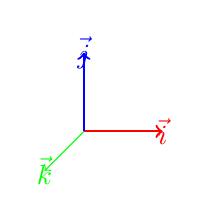
\begin{tikzpicture}

\draw[->, red, thick] (0, 0) -- (1, 0) node {$\vec{i}$};
\draw[->, blue, thick] (0, 0) -- (0, 1) node {$\vec{j}$};
\draw[->, green] (0, 0) -- (-0.5, -0.5) node {$\vec{k}$};

\end{tikzpicture}

Si 3 vecteurs : $\vec{i}, \vec{j}, \vec{k}$ , $||\vec{i}|| = ||\vec{j}|| = ||\vec{k}||$

et $\vec{i}, \vec{j}, \vec{k}$ sont orthogonaux, alors $\vec{i}, \vec{j}, \vec{k}$ forment une base orthonormée. Tous les vecteurs $\vec{V}$ peuvent etre définis par :
$\vec{V} = V_x\vec{i} + V_y\vec{j} + V_z\vec{k}$ avec $V_x, V_y, V_z$ les composants de V dans ($\vec{i}, \vec{j}, \vec{k}$)

\paragraph{Propriétés} l'expression dans une base orthonormée
\[
	\left\{
		\begin{array}{c}
			\vec{V_1} = V_{1x}\vec{i} + V_{1y}\vec{j} + V_{1z}\vec{k} \\
			\vec{V_2} = V_{2x}\vec{i} + V_{2y}\vec{j} + V_{2z}\vec{k}
		\end{array}
	\right.
\]
\begin{align*}
	\vec{V_1} + \vec{V_2} &=& \vec{C} \\
	\vec{C} &=& (V_{2x} + V_{1x})\vec{i} + (V_{2y} + V_{1y})\vec{j} + (V_{2z} + V_{1z})\vec{k}
\end{align*}

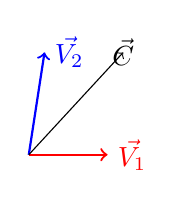
\begin{tikzpicture}
	\draw[->, red, thick] (0, 0) -- (1, 0) node [right] {$\vec{V_1}$};
	\draw[->, blue, thick] (0, 0) -- (0.2, 1.3) node [right] {$\vec{V_2}$};
	\draw[->] (0, 0) -- (1.2, 1.3) node {$\vec{C}$};
\end{tikzpicture}

$\vec{V} = \lambda\vec{V_1}$, les composants sont multipliés par $\lambda$

Si $\vec{V_1} = \vec{V_2}$ alors 
\[
	\left\{
		\begin{array}{c}
			\vec{V_{1x}} = \vec{V_{2x}}\\
			\vec{V_{1y}} = \vec{V_{2y}}\\
			\vec{V_{1z}} = \vec{V_{2z}}
		\end{array}
	\right.
\]

\subsection{Produit Scalaire}
\begin{wrapfigure}[5]{r}{0pt}
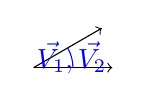
\begin{tikzpicture}
	\draw[->] (0, 0) -- (1, 0);
	\draw[->] (0, 0) -- (30:1);
	\draw[blue] (0.5, 0) arc (0:30:0.5) node [midway] {$\vec{V_1},\vec{V_2}$};
\end{tikzpicture}
\end{wrapfigure}
\begin{align*}
	V &=& \vec{V_1} \cdot \vec{V_2} & \text{Le résultat est un nombre}\\
			&=& ||\vec{V_1}||*||\vec{V_2}||*\cos(\vec{V_1}, \vec{V_2})\\
			&=& (V_{1x}\vec{i} + V_{1y}\vec{j} + V_{1z}\vec{k})*(V_{2x}\vec{i} + V_{2y}\vec{j} + V_{1z}\vec{k}) \\
			&=&	(V_{1x}V_{2x} + V_{1y}V_{2y}+V_{1z}V_{2z}
\end{align*}


Le produit scalaire d'un vecteur par lui meme :

\begin{align*}
			V =& \vec{V_1} \cdot \vec{V_1} & \text{Le résultat est un nombre}\\
	=& V_{1x}^2 + V_{1y}^2 + V_{1z}^2 \\
	=& ||\vec{V_1}||*||\vec{V_1}||\cos(\vec{V_1}, \vec{V_1}) \\
	=& \sum V_{1i}^2 & i=x, y, z
\end{align*}


\[
	\left\{
		\begin{array}{rlr}
			\vec{V_1} \cdot \vec{V_2} &= 0 & \vec{V_1}, \vec{V_2} \text{non nulle} \\
			||\vec{V_1}||*||\vec{V_2}||\cos(\vec{V_1}, \vec{V_2}) &= 0 \\
			\cos((\vec{V_1}, \vec{V_2}) &= 0 \\
			(\vec{V_1}, \vec{V_2}) &= \frac{\pi}{2} \\
		\end{array}
	\right.
\]

Si $\vec{V_1}$ perpendiculaire à $\vec{V_2}$, alors $\vec{V_1}\cdot\vec{V_2} = 0$

\subsection{Produit Vectorielle}

$\vec{V} = \vec{V_1} \wedge \vec{V_2} = ||\vec{V_1}||*||\vec{V_2}||*\sin(\vec{V_1}, \vec{V_2})*\vec{u}$

\begin{wrapfigure}[5]{r}{0pt}
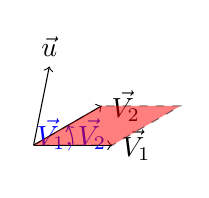
\begin{tikzpicture}
	\draw[->] (0, 0) -- (1, 0) node [right] {$\vec{V_1}$};
	\draw[->] (0, 0) -- (30:1) node [right] {$\vec{V_2}$};
	\draw[->, blue] (0.5, 0) arc (0:30:0.5) node [midway] {$\vec{V_1},\vec{V_2}$};
	\draw[dashed, opacity=0.5, fill=red] (0, 0) -- (30:1) --++ (1, 0) --++(-150:1) --cycle;
	\draw[->] (0, 0) -- (0.2, 1) node [above] {$\vec{u}$};
\end{tikzpicture}
\end{wrapfigure}
~\\

\begin{align*}
\vec{V} &\perp \vec{V_1} \\
	\vec{V} &\perp \vec{V_2}
\end{align*}

Si $\vec{V_1} // \vec{V_2}$ alors $\sin(\vec{V_1}, \vec{V_2}) = 0$ et $\vec{V_1} \wedge \vec{V_2} = \vec{0}$

\paragraph{Composantes du produit vectorielle}
~\\
$\vec{V} = \vec{V_1} \wedge \vec{V_2} = 
	\left(
		\begin{array}{rl}
		V_{1x} & V_{2x} \\
		V_{1y} & V_{2y} \\
		V_{1z} & V_{2z}
		\end{array}
	\right)$
$	\begin{array}{c}
		\vec{i} \\
		\vec{j} \\
		\vec{k} \\

	\end{array}$
	$=
	\begin{array}{c}
		(V_{1y} * V_{2z})-(V_{2y}*V_{1z}) + \\
		(V_{1z}*V_{2x} - V_{2z}*V_{1x}) + \\
		(V_{1x}*V_{2y} - V_{2x}*V_{1y}) 
	\end{array}$

\section{Lois de la statique}

\begin{wrapfigure}[5]{r}{0pt}
	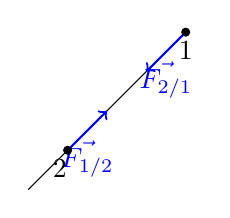
\begin{tikzpicture}
		\draw (0, 0) -- (2, 2);
		\draw[->, blue, thick] (2, 2) -- (1.5, 1.5) node [midway, below] {$\vec{F_{2/1}}$};
		\draw[->, blue, thick] (0.5, 0.5) -- (1, 1) node [midway, below] {$\vec{F_{1/2}}$};
		\draw[fill=black] (0.5, 0.5) circle (0.05) node [xshift=-0.1cm, below] {$2$};
		\draw[fill=black] (2, 2) circle (0.05) node [below] {$1$};
	\end{tikzpicture}
\end{wrapfigure}
Un ensemble de points matériels soumis à des forces est en équilibre statique ou immobile alors 
\begin{itemize}
	\item[1ere lois de la statique :] $\sum(\vec{F}) = \vec{0}$
	\item[2ème lois :] Soit 2 systèmes 1, 2 en interaction mutuelles. La force exercé par 1 sur 2 est égale à l'inverse de la force exercé par 2 sur 1 (meme direction, meme norme, sens opposé)
		$\overrightarrow{F_{1/2}} = - \overrightarrow{F_{2/1}}$
\end{itemize}

$\vec{F_{1/2}}$ s'exerce en 2, et $\vec{F_{2/1}}$ s'applique en 1.

		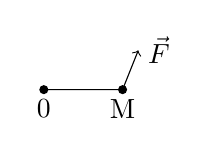
\begin{tikzpicture}
			\draw[fill=black] (0, 0) circle (0.05) node [below] {0} -- (1, 0) circle (0.05) node [below] {M};
			\draw[->] (1, 0) -- (1.2, 0.5) node [right] {$\vec{F}$};
		\end{tikzpicture}

		Le moment de $\vec{F}$ par rapport à O est égale à :
		$\overrightarrow{M_0(\vec{F})}  = \overrightarrow{OM} \wedge \vec{F}$
		Loi de la statistique en rotation dit qu'il existe un point P par rapport auquel $\sum(\overrightarrow{M_P(\vec{F_i})}) = \vec{0}$
		Le moment d'une force est la capacité de cette force à faire tourner un objet au niveau du point d'étude.

		\paragraph{Exemple}
\begin{wrapfigure}{r}{0pt}
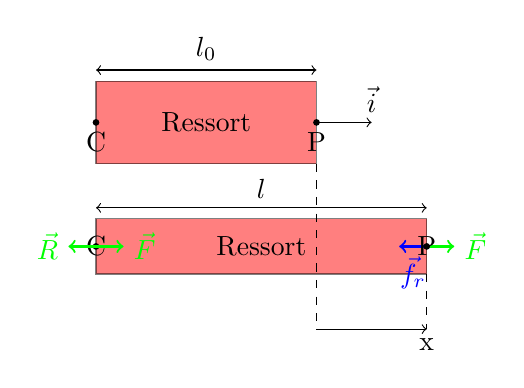
\begin{tikzpicture}[scale=0.7]
	\draw[fill=red, opacity=0.5] (0, 1.5) rectangle (4, 0);
	\node at (2, 0.75) {Ressort};
	\draw[<->] (0, 1.7) -- (4, 1.7) node [midway, above] {$l_0$};
	\draw[->] (4, 0.75) -- (5, 0.75) node [above] {$\vec{i}$};
	\draw[fill=black] (0, 0.75) circle(0.05) node [below] {C};
	\draw[fill=black] (4, 0.75) circle(0.05) node [below] {P};

	\draw[fill=red, opacity=0.5] (0, -1) rectangle (6, -2);
	\draw[<->] (0, -0.8) -- (6, -0.8) node [midway, above] {$l$};
	\draw[->] (4, -3) -- (6, -3) node [below] {x};
	\node at (3, -1.5) {Ressort};
	\draw[->, green, thick] (6, -1.5) -- (6.5, -1.5) node [right] {$\vec{F}$};
	\draw[->, blue, thick] (6, -1.5) -- (5.5, -1.5) node [midway, below] {$\vec{f_r}$};
	\draw[dashed] (4, 0) -- (4, -3);
	\draw[dashed] (6, -2) -- (6, -3);
	\draw[fill=black] (0, -1.5) circle(0.05) node {C};
	\draw[fill=black] (6, -1.5) circle(0.05) node {P};
	\draw[thick, green, ->] (0, -1.5) -- (0.5, -1.5) node [right] {$\vec{F}$};
	\draw[thick, green, ->] (0, -1.5) -- (-0.5, -1.5) node [left] {$\vec{R}$};
\end{tikzpicture}
\end{wrapfigure}

\begin{itemize}
	\item[] Quelles force appliqué en P est nécessaore pour que le système soit en équilibre?
	\item[] Quelles est la force en C pour que le système reste fixe en C ? ~\\
\end{itemize}

\begin{itemize}
	\item[] $\sum\vec{F} = \vec{0}$ en P
		Bilan des forces en P : $\vec{F}, \vec{f_r}$
		~\\
		Expression des forces : \begin{align*}
			\vec{f_r} =& k(l-l_0)(\vec{i}) \\
			=& -kx\vec{i}
		\end{align*}
		~\\
		Application de la loi de la \ul{statique}
		\begin{align*}
			\vec{F} + \vec{f_r}  =& \vec{0} \\
			\vec{F} =& -\vec{f_r} \\
			=& -(-kx\vec{i}) \\
			=& kx\vec{i}
		\end{align*}
		~\\
		Bilan des forces en C : \begin{align*}\vec{F}+\vec{R}=&\vec{0} \\
		\vec{R} =& - \vec{F} = -(-\vec{f_r}) = -kx\vec{i} \\
		\vec{R} =& -kx\vec{i}
	\end{align*}
\end{itemize}
